\section{Compute Disparity}
\label{compute_disparity}

 So far we have learned the essential equations to extract 3D information
from a stereo pair. However, we were faced with some unknown parameters that we have to estimate. 

In this section we will learn how to estimate these missing parameters such as the disparity through
stereo matching. We will also learn that efficient disparity estimation is possible due to epipolar
constraints. 

\begin{framed}
\begin{remark}{\textbf{Epipolar Geometry}}

See the wikipedia article at \url{https://en.wikipedia.org/wiki/Epipolar_geometry}
for epipolar geometry. See also the OpenCV article at \url{https://docs.opencv.org/3.4.3/da/de9/tutorial_py_epipolar_geometry.html}
and the following videos on Coursera

\begin{itemize}
\item \url{https://www.coursera.org/lecture/robotics-perception/epipolar-geometry-i-oNHO9}
\item \url{https://www.coursera.org/lecture/robotics-perception/epipolar-geometry-ii-WRyoL}
\item \url{https://www.coursera.org/lecture/robotics-perception/epipolar-geometry-iii-Bwk0d}
\end{itemize}

\end{remark}
\end{framed}


Recall from section \ref{visual_depth_perception}
that we identified two primary issues with the visual depth estimation from stereo images. 

\begin{itemize}
\item The camera parameters focal length $f$ baseline $b$ 
\item The camera pixel centers $u_0, v_0$
\end{itemize}

These need to be estimated from stereo camera calibration. Similar to monocular
camera calibration, stereo calibration is a well-studied problem with lots of user-friendly
free software capable of performing in. In this section we will be
targeting the second problem, mainly stereo matching
to compute disparities. As a reminder, disparity is the difference in
the image location of the same 3D point as observed
by two different cameras. 

\subsection{Disparity Computation Algorithm}
\label{disparity_computation}

Before we begin let us explain what do we mean with the term disparity


\begin{framed}
\begin{definition}{\textbf{Disparity}}

With the term  disparity we mean the difference in image location of the
same 3D point under perspective to two different cameras.
\end{definition}
\end{framed}

To compute the disparity we need to be able to find the same point in the left and right stereo camera images. 
In other words, we need to find $\mathbf{x}_R$ for each corresponding $\mathbf{x}_L$.
This problem is known as the \textbf{stereo correspondence problem}. 


\begin{framed}
\begin{remark}{\textbf{The Stereo Correspondence Problem}}


\end{remark}
\end{framed}

The simplest solution, however naive one,  for this problem is
an exhaustive search i.e  we search the whole right image for every pixel in the left image. Such a solution is extremely
inefficient and will usually not perform in real time to be used on self-driving cars. It is also unlikely to succeed as many pixels will have
similar local characteristics, making it difficult to match them correctly. Luckily for us, we can use stereo geometry 
to constrain our search problem from 2D over the entire image space to a 1D line. 

Let us revisit the stereo camera setup and see why such a
simplification is valid. We have already determined, how a single point is
projected to both cameras. Now, let's move our 3D point along the line connecting it with the left cameras center. 
Its projection on the left camera image plane does not change. However, what can
you notice about the projection on the right camera plane, the projection moves along the horizontal line. 
This is called an \textbf{epipolar line}, see Figure \ref{epipolar_line}.

\begin{figure}[!htb]
\begin{center}
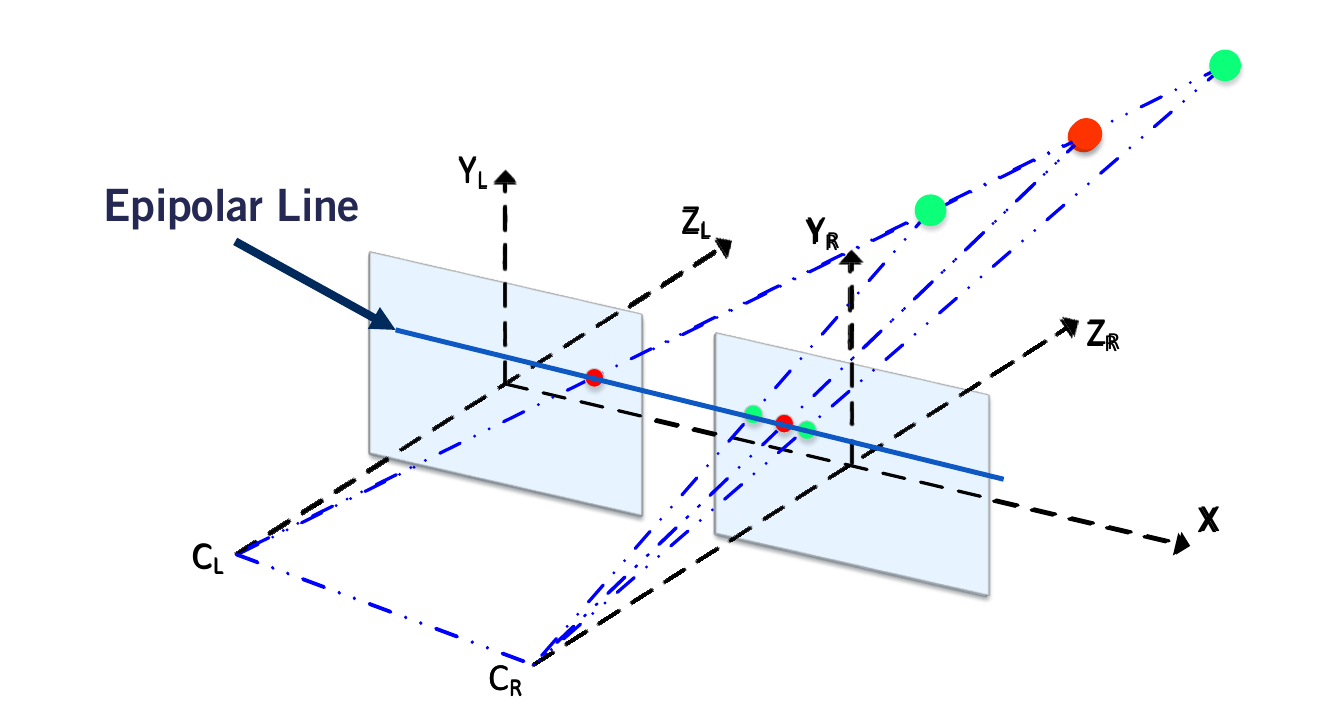
\includegraphics[scale=0.380]{img/visual_perception/epipolar_line.jpeg}
\end{center}
\caption{Epipolar line.}
\label{epipolar_line}
\end{figure}



The epipolar line follows directly from the fixed lateral offset and image plane alignment of the two cameras in a stereo pair. 
We can constrain our correspondence search to be along the epipolar line, reducing the search from 2D to 1D. One thing to note is that
horizontal epipolar lines only occur if the optical axes of the two cameras are parallel. In the case of
non parallel optical axis, the epipolar lines are skewed. In such cases we will
have to result to multiple view geometry rather than the stereo equations we have developed.  

In the case of two calibrated cameras, such as our stereo camera, a skewed epipolar line
is not a huge problem. In fact, we can work the optical axis to be parallel through a process
known as \textbf{stereo rectification}. After rectification we arrive back to our horizontal
epipolar line. We will not go through how to perform rectification
as implementations are available in standard
computer vision packages such as OpenCV and MATLAB. 


\begin{framed}
\begin{remark}{\textbf{Stereo Rectification}}

See the following article on wikipedia about image rectification \url{https://en.wikipedia.org/wiki/Image_rectification}.
Also OpenCV base stereo image calibration \url{https://sourishghosh.com/2016/stereo-calibration-cpp-opencv/}.
\end{remark}
\end{framed}

Let us go over our first basic stereo algorithm.

\begin{enumerate}
\item For each epipolar line take a pixel on this line in the left image
\item Compare these left image pixels to every pixel in the right image on the same epipolar line. 
\item Pick the pixel that has minimum cost. For example, a very simple cost here can be the squared difference in pixel intensities.
\item Compute disparity $d$ by subtracting the right image location from the left one
\end{enumerate}

Stereo matching is a very well-studied problem
in computer vision. Many more complex costs and search regions can be defined, which attempts to improve either computational efficiency
or disparity accuracy. There are a wide range of approaches including both local
and global methods, which differ in the main image region considered when identifying correspondences
and computing disparities. As with most problems in computer vision, the stereo vision algorithms are evaluated 
on a public benchmark. The most famous of which is the Middlebury stereo benchmark, \url{ http://vision.middlebury.edu/stereo/eval3/}. 
If you are interested, many of the top-performing
stereo matching algorithms have results published there
and have code available too. 

\subsection{Summary}

\subsection{Questions}

\subsection{Assignements}
